\documentclass[11pt]{article}\usepackage[]{graphicx}\usepackage[]{color}

\usepackage{alltt}
\usepackage[margin=1in]{geometry}   % set up margins
\usepackage[T1]{fontenc}
\usepackage{enumerate}              % fancy enumerate
\usepackage{amsmath}
\usepackage{amsthm}
\usepackage{amssymb}              % used for \eqref{} in this document
\usepackage{verbatim}               % useful for \begin{comment} and \end{comment}
\usepackage{eurosym}                % used for euro symbol
\usepackage{tabularx}
\usepackage{caption} 
\usepackage{graphicx}
\graphicspath{{Figures/}}
\usepackage{subcaption}
\usepackage[para,online,flushleft]{threeparttable}
\usepackage[usenames,dvipsnames]{xcolor}
\usepackage[colorlinks=true]{hyperref}
\hypersetup{colorlinks=true, citecolor=ForestGreen, linkcolor=BlueViolet, urlcolor=Magenta}
\usepackage{indentfirst}
\usepackage{hyperref}
\usepackage{booktabs}
\usepackage{tabularx}
\usepackage{mathrsfs}
\usepackage{dsfont}
\usepackage{float}
\usepackage{pgfplots}
\usepackage[draft]{todonotes} 
\usepackage{soul}
\newcommand{\hlc}[2][yellow]{ {\sethlcolor{#1} \hl{#2}} }
\setlength\parindent{0pt}


%Folders
\graphicspath{ {/Users/andreaotero/Documents/GitHub/prueba/RDD/Figures/} }




\begin{document}


\title{\textbf{Homework 4} }
\date{June 12 2020}

\maketitle

Name: Andrea Otero Cortes {\hspace{4.5cm}}



\subsection*{Questions}

\begin{enumerate} 

\item  \href{https://github.com/aoteroco/RDD}{GitHub Repo}
\item \textbf{Summary Hansen (2015)}:
\newline
 The paper studies the effect of additional sanctions on drunk drivers on reducing repeated DUI incidents using a local linear regression discontinuity design. 
 The author uses an RDD setting as drunk-driving sanctions in Washington State are determined by strict thresholds on the blood alcohol content test (BAC) that allows police officers to classify drivers as above the DUI limit or above the aggravated DUI limit and impose sanctions and fines depending on it. The punishment is harsher for severely intoxicated drivers and repeated offenders, even including jail time. The data comes from administrative records on 512.964 DUI stops from Washington State. Specifically, a BAC measured above 0.08 is considered a DUI and a BAC over 0.15 is considered an aggravated DUI.
 \newline
 The results indicate that the punishment on offenders whose BAC is above the DIU limit reduces recidivism by 2 percentage points. The additional sanctions for having a BAC over the aggravated DIU threshold reduce recidivism by an additional percentage point. Therefore, the results suggest that the additional sanctions on severely intoxicated drivers are effective in reducing drunk-driving. When looking at the mechanisms for these results, the author argues that deterrence seems to be the main one, although he cannot rule out other potential mechanism such as incapacitation and rehabilitation.
 
 \item  $gen \; dui= (bac1>=0.08)$

 
 \item In order to test if individuals or police officers were able to manipulate the running variable, which in this case is the BAC test, we would have to do a density test to see if there is evidence of bunching right before the cutoff or threshold for getting a DUI, which is 0.08  (or in case of an aggravated DUI, which is 0.15).
 
Although the visual inspection of the historgram of the BAC test presented in the paper does not show evidence of bunching, based on the bias-corrected McCrary test, we find slight evidence of manipulation of the BAC at 5\% around the 0.08 cutoff (Figure \ref{densitytest}).

 
 \begin{figure}[!htb]
 \centering
  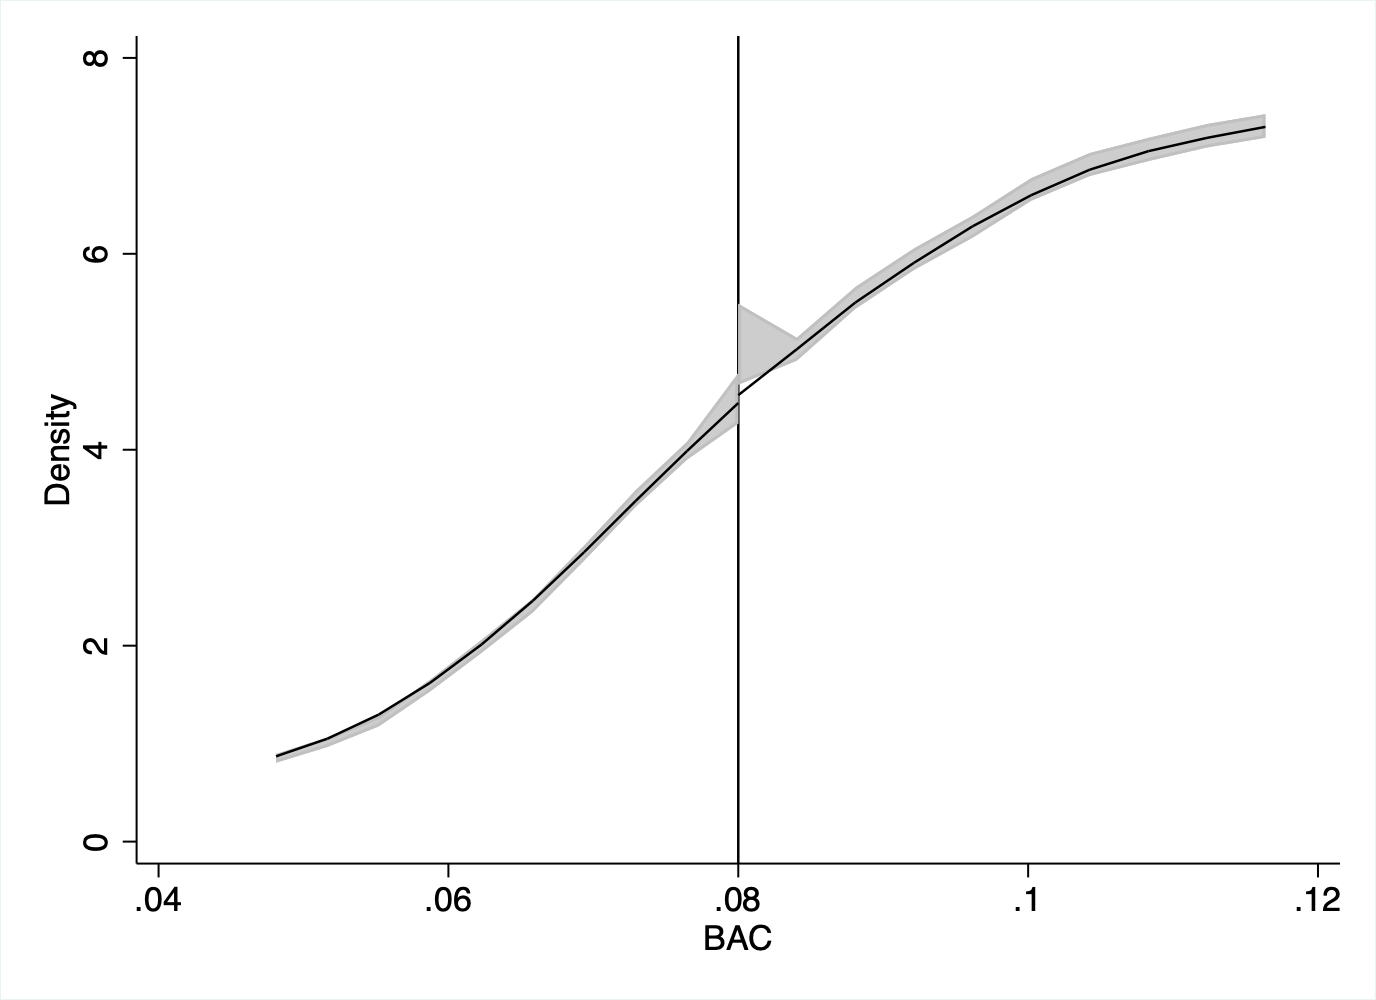
\includegraphics[scale=0.6]{figure1}
\caption{Density Test}
\label{densitytest}
 \end{figure}
 
\item Balance test (Table \ref{table:balancetest})
\newline
The covariates seem to be balanced around the cutoff, when we only consider data +/- 0.05 around the cutoff. Running the same balance test for the whole sample reveals that the covariates ``Male'' and ``Age'' react to the BAC threshold.

 \begin{table}[htbp]\centering
\small
\caption{Regression Discontinuity Estimates for the Effect of Exceeding BAC Thresholds on Predetermined Driver Characteristics}
\label{table:balancetest}
\begin{center}
\begin{threeparttable}
\begin{tabular}{l*{4}{c}}
\toprule
\multicolumn{1}{l}{\textit{Dependent var: }}&
\multicolumn{1}{c}{\textit{Male}}&
\multicolumn{1}{c}{\textit{White}}&
\multicolumn{1}{c}{\textit{Age}}&
\multicolumn{1}{c}{\textit{Accident}}\\
\midrule
\textit{Panel A: $BAC \in [0.075, 0.085]$ } & 		&			& 			& 		\\
DUI                 &      -0.001   &       0.022   &       0.556   &       0.005   \\
                    &     (0.019)   &     (0.016)   &     (0.532)   &     (0.013)   \\
$\tilde{BAC}$              &      -3.963   &      -1.048   &     -81.657   &      -0.721   \\
                    &     (3.261)   &     (2.864)   &    (94.213)   &     (2.278)   \\
Interaction         &       4.280   &      -4.212   &    -122.804   &      -1.338   \\
                    &     (6.731)   &     (5.630)   &   (190.447)   &     (4.503)   \\
			&		&			&		&			\\
Controls   & No			& No			& No 	& No \\
Mean of dependent variable&        0.79   &        0.85   &       34.11   &        0.09   \\
N                   &       9,514   &       9,514   &       9,514   &       9,514   \\
\midrule
\textit{Panel B: Complete sample} & 		&			& 			& 		\\
dui                 &       0.006   &       0.004   &      -1.115***&      -0.007** \\
                    &     (0.004)   &     (0.004)   &     (0.121)   &     (0.003)   \\
$\tilde{BAC}$             &       0.218*  &       0.154   &     -56.361***&      -1.540***\\
                    &     (0.112)   &     (0.098)   &     (3.223)   &     (0.098)   \\
interaction         &      -0.311***&       0.017   &      83.400***&       2.656***\\
                    &     (0.114)   &     (0.099)   &     (3.268)   &     (0.100)   \\
			&		&			&		&			\\
Controls   & No			& No			& No 	& No \\
Mean of dependent variable&        0.79   &        0.86   &       34.96   &        0.15   \\
N                   &     214,558   &     214,558   &     214,558   &     214,558   \\
\bottomrule
\end{tabular}
\begin{tablenotes}
\tiny
\item This table contains regression discontinuity based estimates of the effect of having a BAC above the legal thresholds on predetermined  drivers characteristics based on Hansen (2015). Panel A only includes  observations with a BAC test +/- 0.05 around the 0.08 cutoff. Panel B includes all the data. Heteroskedastic standard errors shown in parenthesis.  * p$<$0.10, ** p$<$0.05, *** p$<$0.01
\end{tablenotes}
\end{threeparttable}
\end{center}
\end{table}



 \item BAC and bins of predetermined drivers' characteristics.
 \newline
 Based on Figure \ref{figure2_all_lfit} and  \ref{figure2_all_qfit}, we find the same results as in Q5: there is a slight discontinuity at the threshold for some of the covariates (dummy for male, age, and dummy for accident), which would suggest a violation of one of the identifying assumptions in the RDD design. This is consistent with the results that Hansen shows in his paper. As I used the whole sample for this question, I get some weird outliers in the graphs. This would disappear if I only use observations for which BAC is less than 0.15.
 \begin{itemize}
 \item Linear fit (Figure \ref{figure2_all_lfit})
 
  \begin{figure}[!htb]
  \caption{BAC and drivers' characteristics (linear fit)}
  \label{figure2_all_lfit}
 \centering
  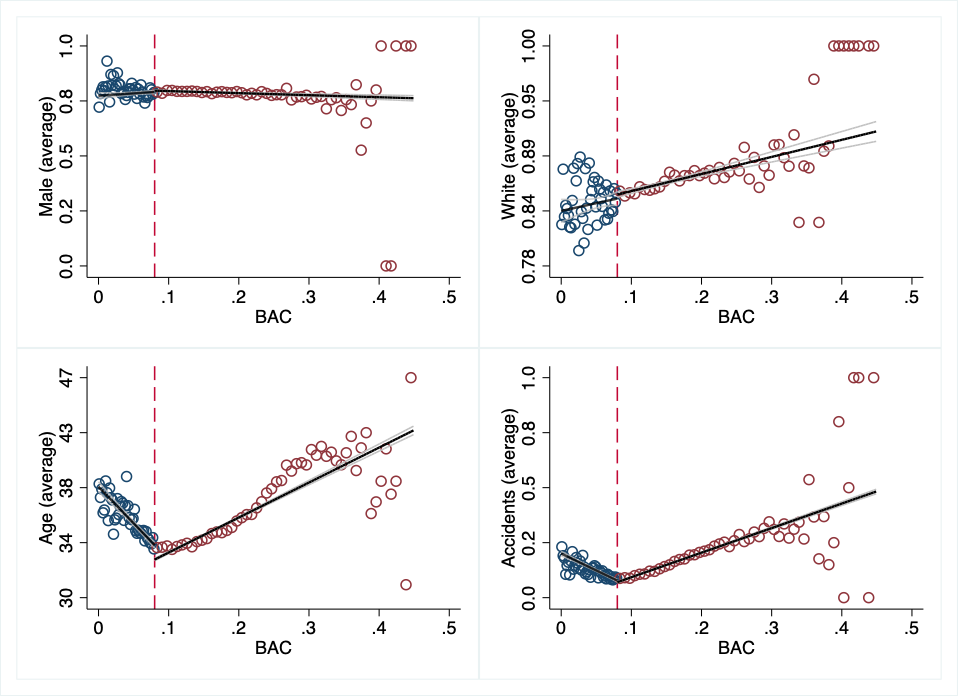
\includegraphics[scale=1]{figure2_all_lfit}
 \end{figure}
 
 \item Quadratic fit (Figure \ref{figure2_all_qfit})
 
   \begin{figure}[!htb]
   \caption{BAC and drivers' characteristics (quadratic fit)}
\label{figure2_all_qfit}
 \centering
  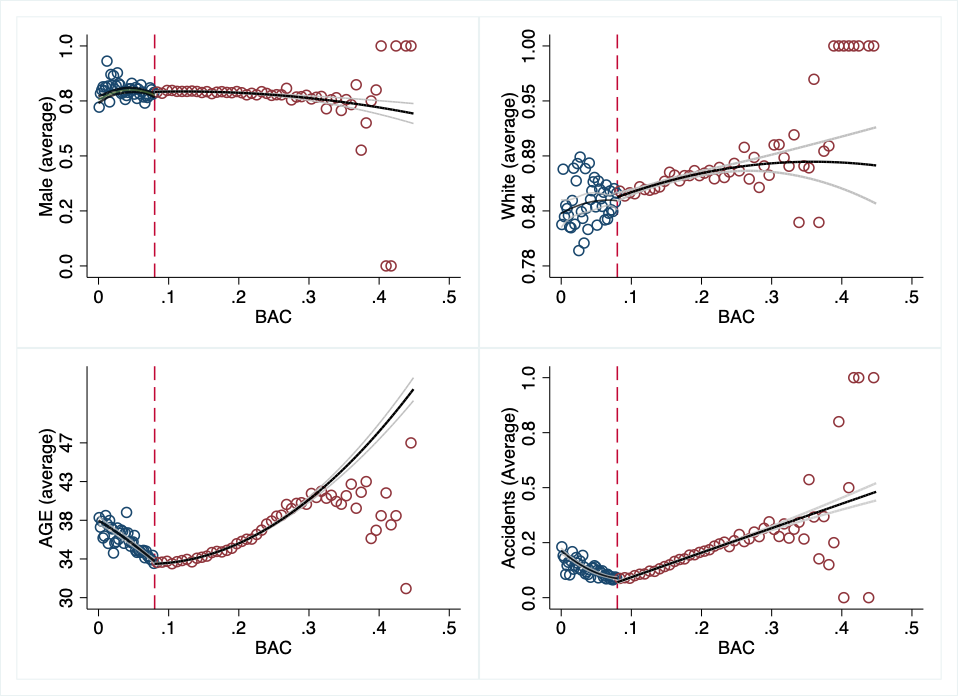
\includegraphics[scale=1]{figure2_all_qfit}
 \end{figure}
 
 \end{itemize}
 
 \item Table \ref{table:mainreg} reports the estimated effect of having BAC over DUI threshold for all the drivers with a BAC within a defined threshold. The results are not identical to Hansen (2015) as we do not have access to all of his covariates, but the coefficient of interest on DUI remains statistically significant and negative. In particular, using a  bandwidth of 0.05 (Panel A), I find that the effect of getting a DUI reduces recidivism between 1.4-2.7 percentage points, depending on the specification of the model. If I use a bandwidth of 0.025, then the effect on recidivism ranges from -1.4 to -2.2 percentage points, depending on the specification of the model. The results are consistent across different bandwidths and are robust to the inclusion of quadratic polynomial and a set of controls like sex, age and race. All the results are very close to what Hansen (2015) finds.
 

\begin{table}[htbp]\centering
\small
\caption{Regression Discontinuity Estimates for the Effect of Exceeding BAC Thresholds on Recidivism}
\label{table:mainreg}
\begin{center}
\begin{threeparttable}
\begin{tabular}{l*{6}{c}}
\toprule
\multicolumn{1}{l}{\textit{Dependent var: }}&
\multicolumn{1}{c}{\textit{(1)}}&
\multicolumn{1}{c}{\textit{(2)}}&
\multicolumn{1}{c}{\textit{(3)}}&
\multicolumn{1}{c}{\textit{(4)}}&
\multicolumn{1}{c}{\textit{(5)}}&
\multicolumn{1}{c}{\textit{(6)}}\\
\midrule
\textit{Panel A: $BAC \in [0.03, 0.13]$ } & & & & & & \\
DUI                 &      -0.027***&      -0.024***&      -0.014** &      -0.027***&      -0.024***&      -0.014** \\
                    &     (0.004)   &     (0.004)   &     (0.006)   &     (0.004)   &     (0.004)   &     (0.006)   \\
$\tilde{BAC}$            &       0.331***&       0.006   &      -1.000*  &       0.323***&      -0.047   &      -1.057*  \\
                    &     (0.075)   &     (0.187)   &     (0.602)   &     (0.075)   &     (0.187)   &     (0.601)   \\
interaction         &               &       0.392*  &       1.016   &               &       0.446** &       1.032   \\
                    &               &     (0.204)   &     (0.690)   &               &     (0.204)   &     (0.689)   \\
$\tilde{BAC}^2$            &               &               &     -24.614*  &               &               &     -24.719*  \\
                    &               &               &    (13.771)   &               &               &    (13.740)   \\
interaction\_sq      &               &               &      31.871** &               &               &      32.778** \\
                    &               &               &    (15.138)   &               &               &    (15.105)   \\
\midrule
Controls   & No			& No			& No 	& Yes 		& Yes 		& Yes  \\
Mean of dependent variable&        0.11   &        0.11   &        0.11   &        0.11   &        0.11   &        0.11   \\
N                   &      89,967   &      89,967   &      89,967   &      89,967   &      89,967   &      89,967   \\
\midrule
\textit{Panel B: $BAC \in [0.055, 0.105]$ } & & & & & &		\\
DUI                 &      -0.022***&      -0.020***&      -0.015*  &      -0.022***&      -0.021***&      -0.014*  \\
                    &     (0.006)   &     (0.006)   &     (0.008)   &     (0.006)   &     (0.006)   &     (0.008)   \\
$\tilde{BAC}$             &       0.216   &      -0.150   &      -0.984   &       0.188   &      -0.199   &      -1.201   \\
                    &     (0.201)   &     (0.383)   &     (1.346)   &     (0.201)   &     (0.383)   &     (1.344)   \\
Interaction         &               &       0.523   &       0.682   &               &       0.552   &       0.879   \\
                    &               &     (0.450)   &     (1.677)   &               &     (0.449)   &     (1.675)   \\
$\tilde{BAC}^2$            &               &               &     -38.124   &               &               &     -45.804   \\
                    &               &               &    (58.838)   &               &               &    (58.762)   \\
Interaction sq.      &               &               &      63.419   &               &               &      71.090   \\
                    &               &               &    (69.302)   &               &               &    (69.218)   \\
\midrule
Controls   & No			& No			& No 	& Yes 		& Yes 		& Yes  \\
Mean of dependent variable&        0.11   &        0.11   &        0.11   &        0.11   &        0.11   &        0.11   \\
N                   &      46,957   &      46,957   &      46,957   &      46,957   &      46,957   &      46,957   \\
\bottomrule
\end{tabular}
\begin{tablenotes}
\tiny
\item This table contains regression discontinuity based estimates of the effect of having BAC above the legal thresholds on recidivism based on Hansen (2015). Panel A contains observations with BAC +/-0.05 around the cutoff. Panel B contains observations with BAC +/-0.025 around the cutoff. Heteroskedastic standard errors shown in parenthesis.  * p$<$0.10, ** p$<$0.05, *** p$<$0.01
\end{tablenotes}
\end{threeparttable}
\end{center}
\end{table}

\newpage
\item BAC and Recidivism.
Figures \ref{figure3_lfit} and \ref{figure3_qfit} plot the means of recidivism rates in bin and predicted recidvisim rates based on a regression model for all the individuals with a BAC less than 0.15. This is graphical evidence of the jump that Hansen (2015) reports after getting a DUI. This shows that there is an important drop in recidivism at the 0.08 BAC threshold, which is the limit that indicates when driver should get a sanction for driving under the influence of alcohol. Hansen (2015) argues that this is evidence that the increase of punishments and sanctions at the threshold is effective in reducing future drunk driving.
 
  \begin{figure}[!htb]
  \caption{BAC and recidivism (linear fit)}
  \label{figure3_lfit}
 \centering
  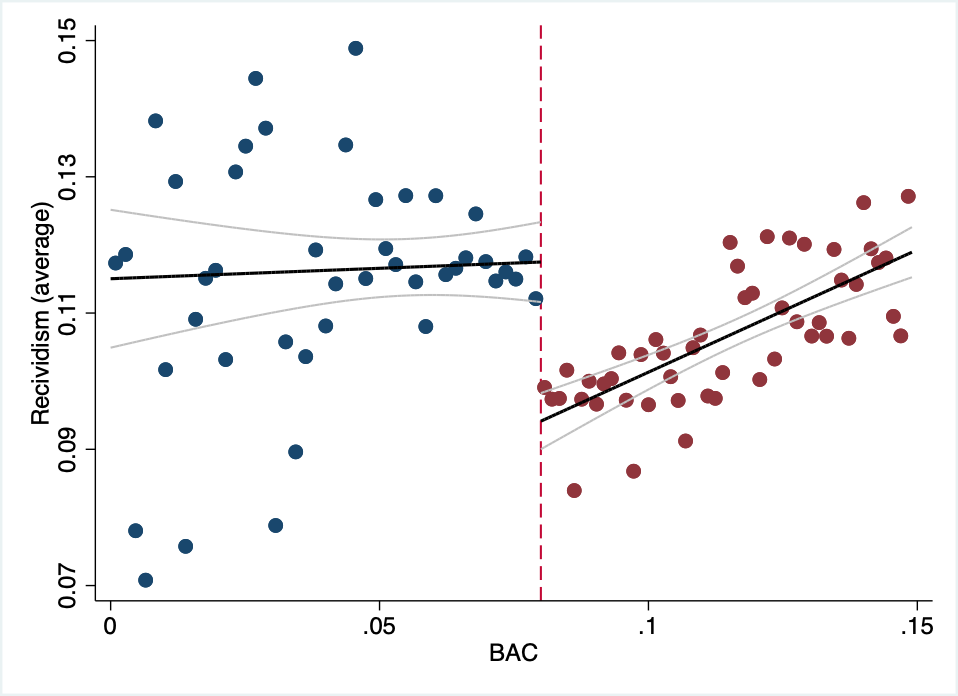
\includegraphics[scale=1]{figure3_lfit}
 \end{figure}
 
  \begin{figure}[!htb]
  \caption{BAC and recidivism (quadratic fit)}
  \label{figure3_qfit}
 \centering
  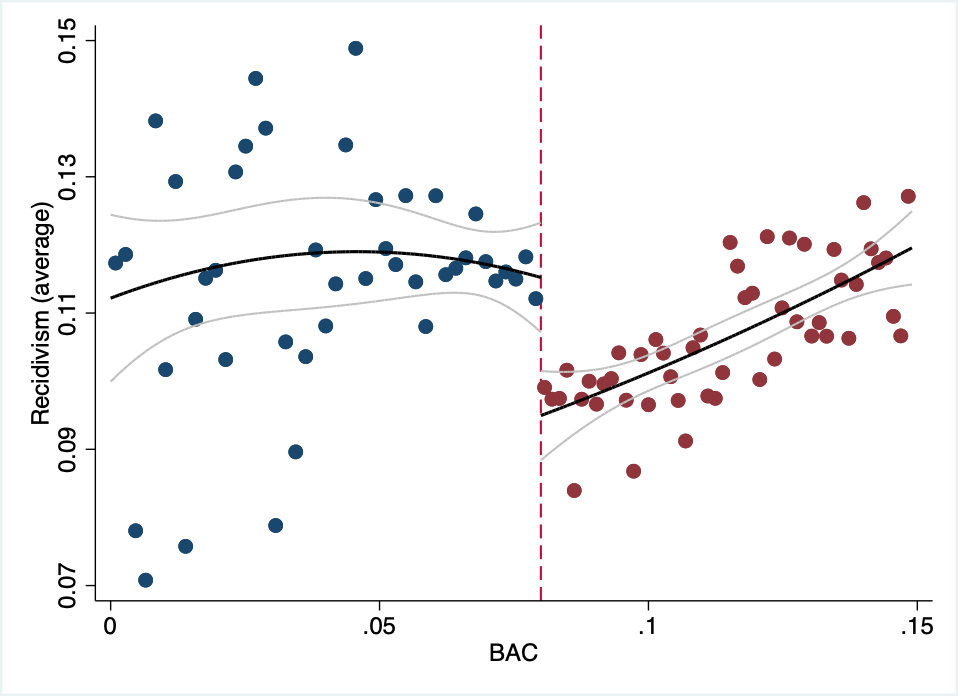
\includegraphics[scale=1]{figure3_qfit}
 \end{figure}
  
 \end{enumerate}

\end{document}

